\begin{figure}[t]
      \centering
      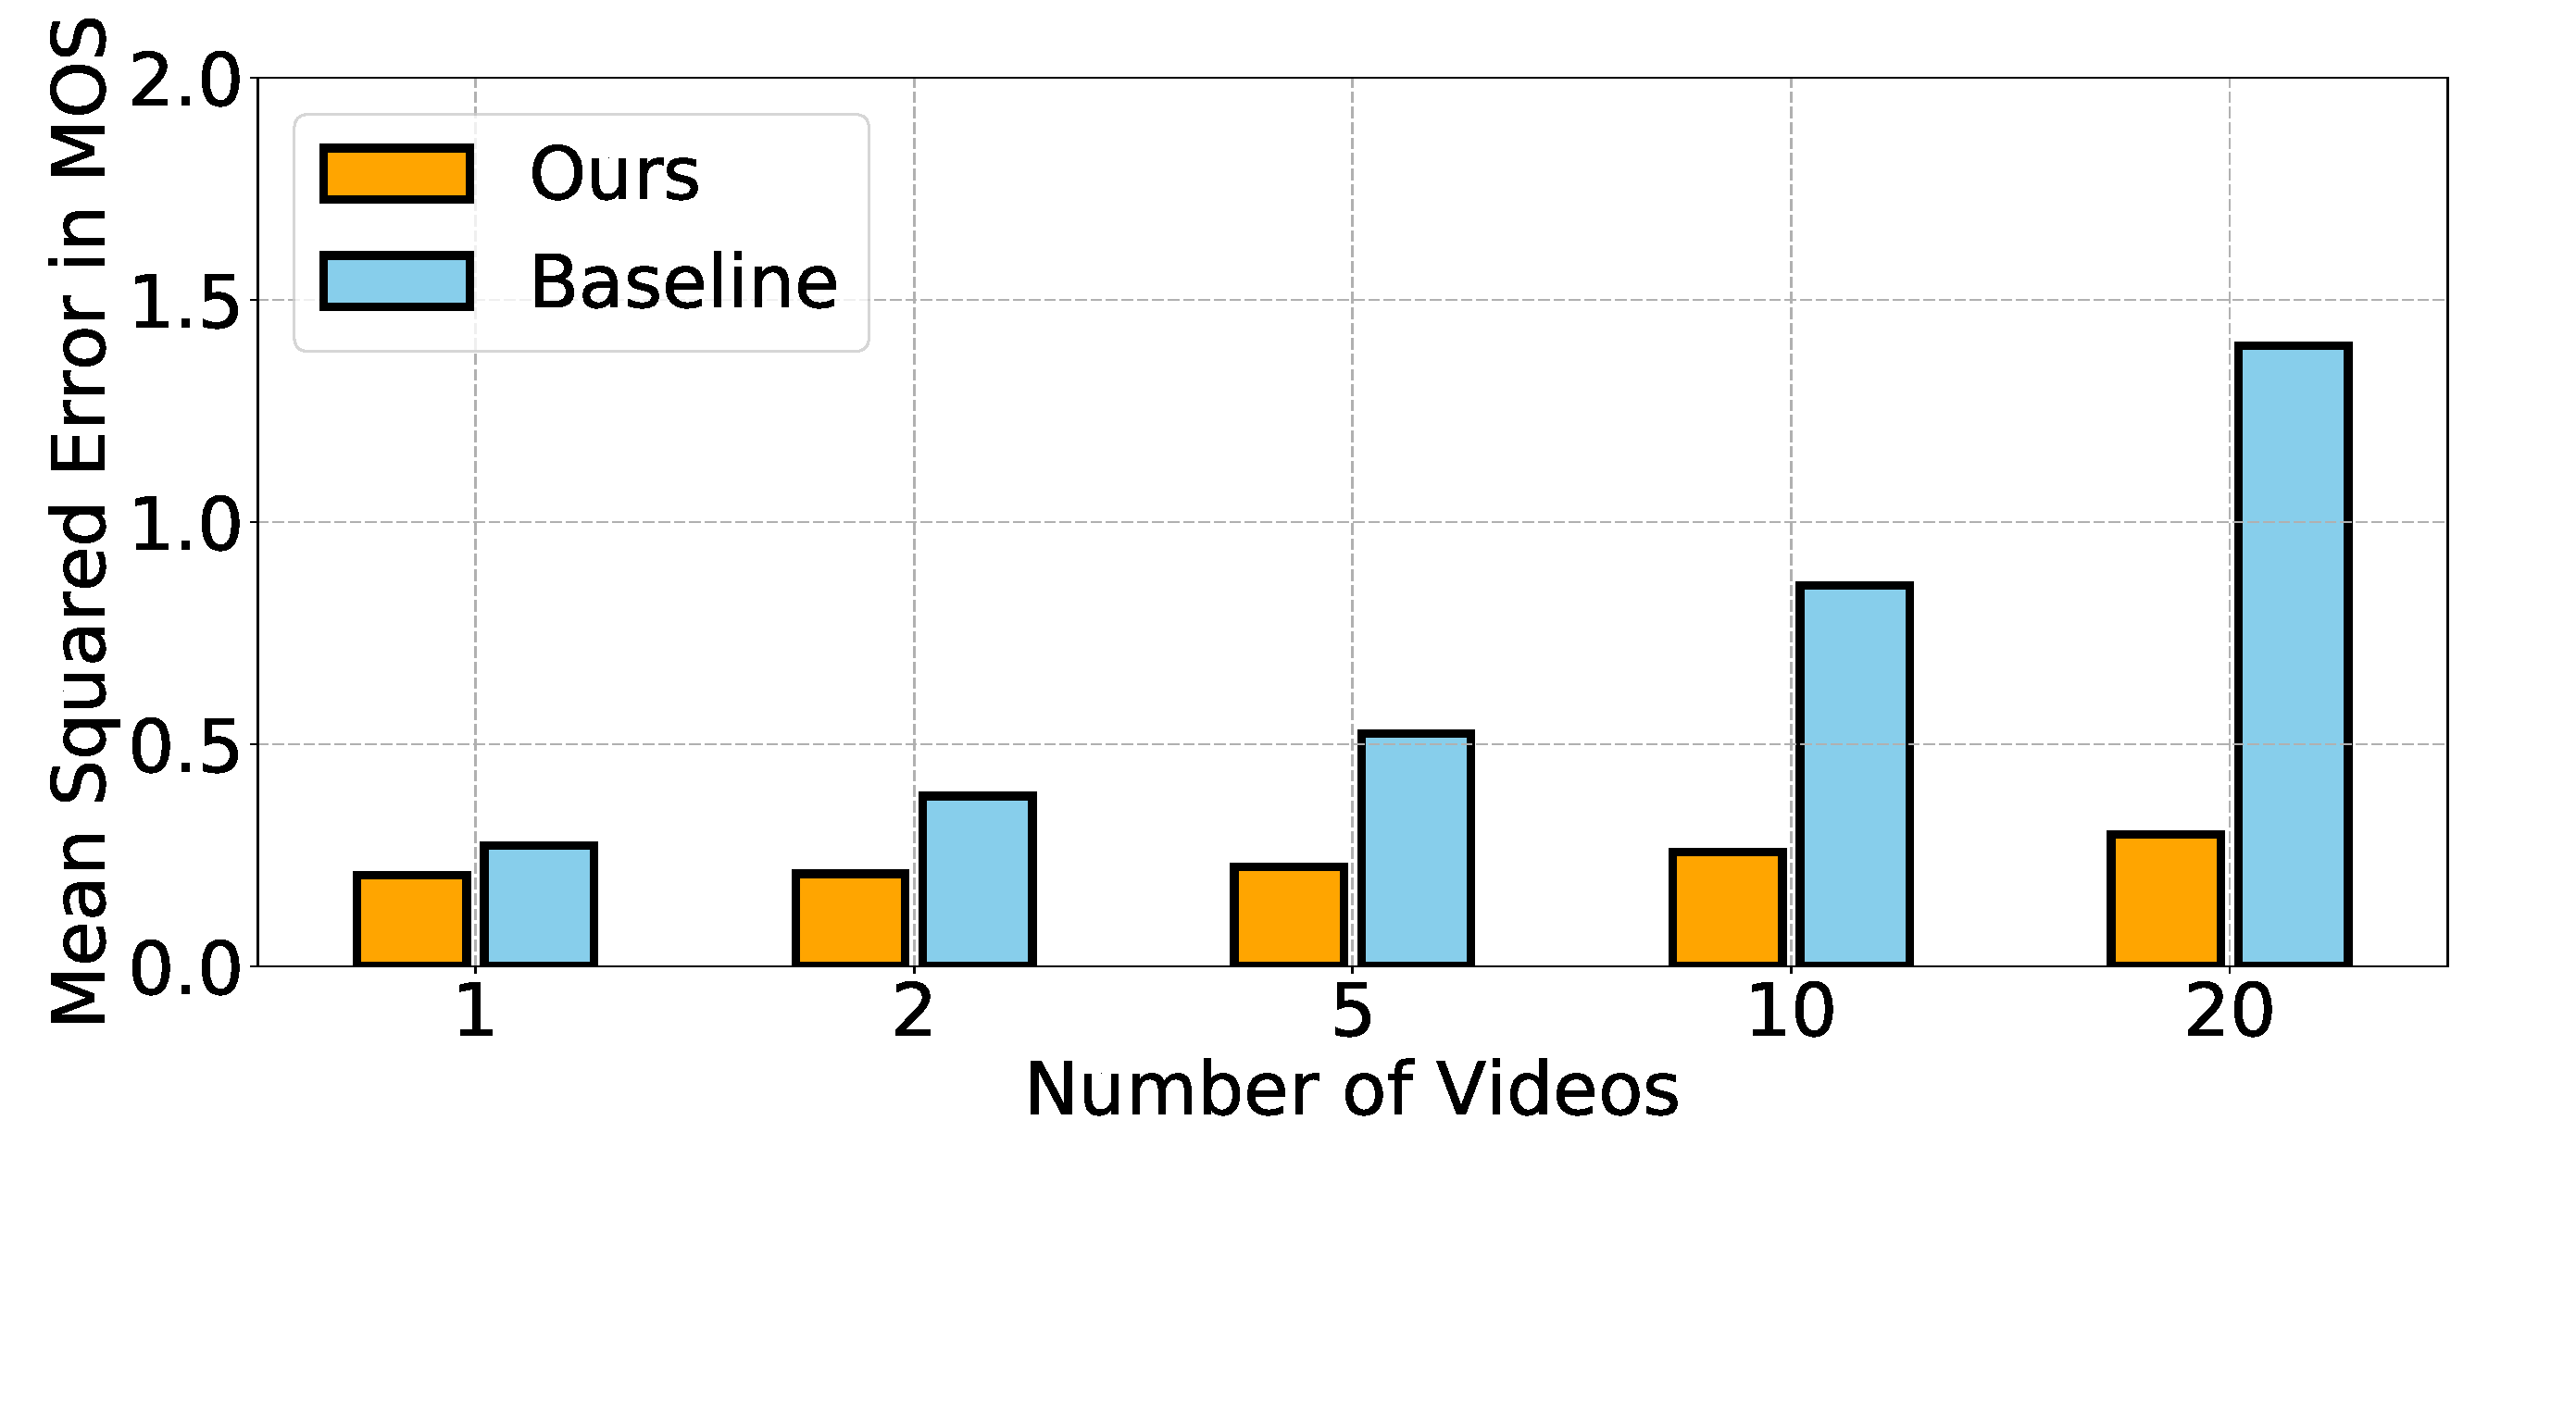
\includegraphics[width=\linewidth]{sections/network-work/baseline}
      \vspace{-3em}
      \caption{Comparison of our metrics vs.~baseline. Baseline has an up to 1.4 MOS estimation error across 20 video contents, hence failing to distinguish good/bad from average QoE. }
      %\vspace{-1.4em}
      \label{fig:baseline}
\end{figure}

\begin{figure}[t]
      \centering
      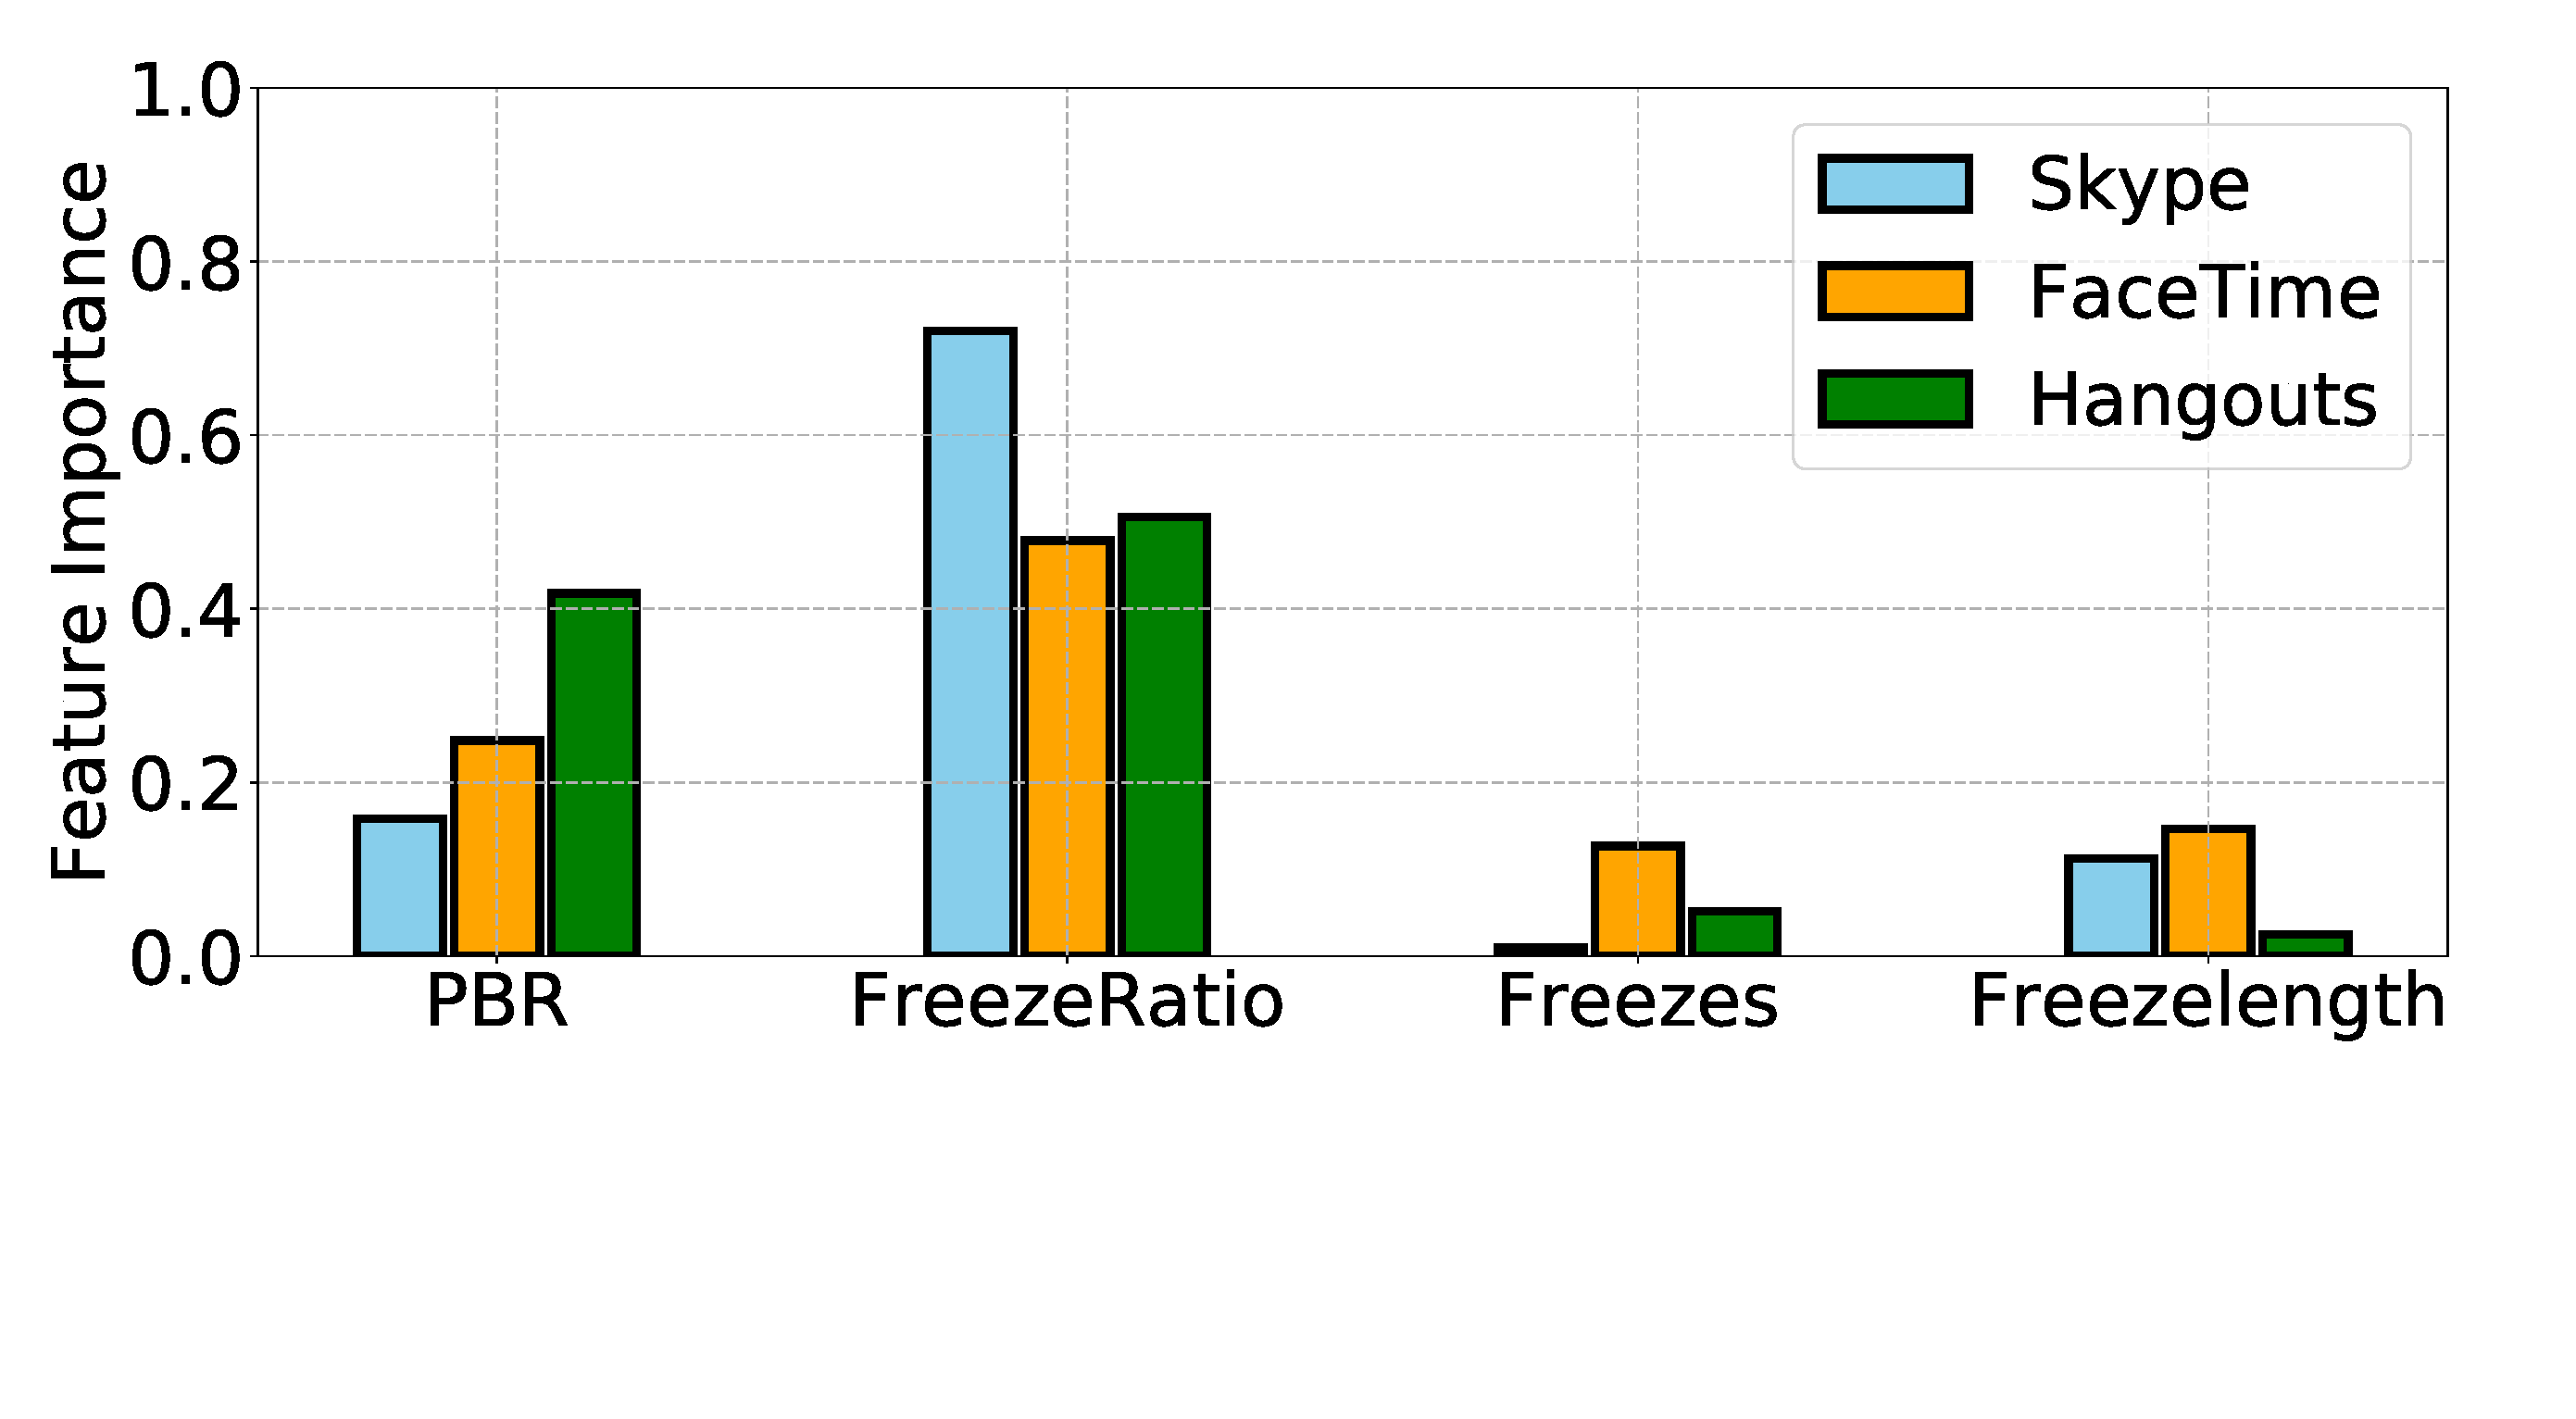
\includegraphics[width=\linewidth]{sections/network-work/feature-imp.pdf}
      \vspace{-4em}
      \caption{Feature Importance for the three applications.}
      %\vspace{-1.0em}
      \label{fig:ft-imp}
\end{figure}

\subsection{Comparison with Baseline and Feature Importance}
We compare our model prediction error with previous work for Skype application. As we need no-reference metrics for the baseline comparison, we use the DCT blur metric used by Jana {\em et al} as spatial metric and frame-drop metric in \cite{usman2017no} as temporal metric. We fit the ADT model with these two metrics as well as with our metrics using the MOS scores from our user-study. Fig. \ref{fig:baseline} shows the performance of Skype application across the 20 videos described in Section \ref{MOTIVATION}. Clearly, for a single video, both baseline and our model yield less than 0.2 MSE in MOS whereas as the number of videos increases, the MSE grows larger than 1.3 MOS for baseline metrics. Whereas, our model has a maximum of 0.4 MSE. The baseline metric's high MOS error with large number of videos is due to DCT metric's inability to scale across diverse video content. In fact, in our experiments we measure feature importance, which is defined as the amount each feature improves performance weighted by the number of samples this feature is responsible for. We observe that feature importance for DCT is as low as $0.1$, and it is $0.9$ for frame-drop metric. Therefore, previous metrics fail to model video telephony QoE across diverse videos. We observe similar results for FaceTime and Hangouts.

We also evaluate the importance of each proposed metric. Fig. \ref{fig:ft-imp} shows the importance of features for ADT over all three applications. Out of all features, freeze ratio is dominating with at least $0.5$ feature importance on all applications. For Skype, we observe highest ($>0.7$) importance to freeze ratio. The rest of the metrics are almost equally important, and removal of any of these features causes an up to 0.2 accuracy degradation. Whereas, for FaceTime and Hangouts, we notice high importance for PBR ($0.28$ for FaceTime and $0.41$ for Hangouts) due to their compromise in quality over freezes.

